\documentclass[UTF8,a4paper,11pt,fontset=fandol]{ctexart}

\usepackage[left=2.15cm,right=2.15cm,top=2.25cm,bottom=2.15cm,headsep=0.7cm]{geometry}
\usepackage{amsmath,amssymb}
\usepackage{booktabs}
\usepackage{array}
\usepackage{tabularx}
\usepackage{longtable}
\usepackage{enumitem}
\usepackage{xcolor}
\usepackage{graphicx}
\usepackage{tikz}
\usetikzlibrary{arrows.meta,positioning,calc,shapes.geometric}
\usepackage{tcolorbox}
\tcbuselibrary{breakable}
\usepackage{needspace}
\numberwithin{equation}{subsection}
\renewcommand{\theequation}{\arabic{section}.\arabic{subsection}.\arabic{equation}}
\usepackage{hyperref}

\definecolor{Ink}{HTML}{17233C}
\definecolor{Navy}{HTML}{173B68}
\definecolor{Blue}{HTML}{2878B5}
\definecolor{Cyan}{HTML}{2A9D8F}
\definecolor{Amber}{HTML}{E9A23B}
\definecolor{Red}{HTML}{C84B4B}
\definecolor{Paper}{HTML}{F6F8FB}
\definecolor{PaleBlue}{HTML}{EAF2FA}
\definecolor{PaleCyan}{HTML}{EAF7F4}
\definecolor{PaleAmber}{HTML}{FFF5E4}
\definecolor{Rule}{HTML}{D6DEE8}
\definecolor{Muted}{HTML}{5B677A}

\hypersetup{
  colorlinks=true,
  linkcolor=Navy,
  urlcolor=Blue,
  citecolor=Cyan,
  pdfauthor={钟志诚（主讲）；曾有成（整理）},
  pdftitle={第二次实验讲义：从二叉树到决策树},
  pdfsubject={二叉树、二叉搜索树、决策树推理、信息熵、信息增益与西瓜分类}
}

\ctexset{
  section={
    format=\Large\bfseries\color{Navy},
    number=\chinese{section},
    name={第,部分},
    aftername=\quad,
    beforeskip=1.4ex plus .2ex,
    afterskip=.8ex
  },
  subsection={
    format=\large\bfseries\color{Ink},
    beforeskip=1.2ex plus .2ex,
    afterskip=.55ex
  },
  subsubsection={
    format=\normalsize\bfseries\color{Blue},
    beforeskip=1ex,
    afterskip=.35ex
  }
}

\setlength{\parindent}{2em}
\setlength{\parskip}{0.22em}
\setlength{\emergencystretch}{2em}
\linespread{1.16}
\setlist[itemize]{leftmargin=2em,itemsep=.25em,topsep=.35em}
\setlist[enumerate]{leftmargin=2.2em,itemsep=.28em,topsep=.35em}
\renewcommand{\arraystretch}{1.34}

\newcolumntype{Y}{>{\raggedright\arraybackslash}X}
\newcolumntype{C}[1]{>{\centering\arraybackslash}p{#1}}
\newcolumntype{L}[1]{>{\raggedright\arraybackslash}p{#1}}

\newcommand{\R}{\mathbb{R}}
\newcommand{\E}{\operatorname{E}}
\newcommand{\Var}{\operatorname{D}}
\newcommand{\Cov}{\operatorname{Cov}}
\newcommand{\MSE}{\operatorname{MSE}}
\newcommand{\RMSE}{\operatorname{RMSE}}
\newcommand{\argmin}{\operatorname*{arg\,min}}
\newcommand{\argmax}{\operatorname*{arg\,max}}
\newcommand{\vect}[1]{\boldsymbol{#1}}
\newcommand{\mat}[1]{\mathbf{#1}}
\newcommand{\diff}{\mathop{}\!\mathrm{d}}
\newcommand{\term}[1]{\textcolor{Blue}{\textbf{#1}}}
\newcommand{\dimtag}[1]{\textcolor{Muted}{\scriptsize$#1$}}

\tcbset{
  boxrule=.7pt,
  arc=1.6mm,
  left=2.5mm,right=2.5mm,top=1.8mm,bottom=1.8mm,
  before skip=7pt,after skip=7pt,
  breakable
}
\newtcolorbox{keybox}[1][核心结论]{
  colback=PaleBlue,colframe=Blue,
  title={#1},fonttitle=\bfseries,coltitle=white
}
\newtcolorbox{examplebox}[1][贯穿例题]{
  colback=PaleCyan,colframe=Cyan,
  title={#1},fonttitle=\bfseries,coltitle=Ink
}
\newtcolorbox{questionbox}[1][思考题]{
  colback=PaleAmber,colframe=Amber,
  title={#1},fonttitle=\bfseries,coltitle=Ink
}
\newtcolorbox{pitfallbox}[1][易错提醒]{
  colback=red!3,colframe=Red,
  title={#1},fonttitle=\bfseries,coltitle=white
}
\newtcolorbox{notebox}[1][实现约定]{
  colback=Paper,colframe=Rule,
  title={#1},fonttitle=\bfseries,coltitle=Muted
}
\newtcolorbox{proofbox}[1][推导与证明]{
  colback=Blue!3,colframe=Navy,
  title={#1},fonttitle=\bfseries,coltitle=white
}

\makeatletter
\def\ps@lesson{
  \def\@oddhead{\hbox to\textwidth{\small\color{Muted}人工智能数学原理与算法\hfil 实验02：从二叉树到决策树}}
  \def\@evenhead{\@oddhead}
  \def\@oddfoot{\hbox to\textwidth{\small\color{Muted}实验讲义\hfil\thepage}}
  \def\@evenfoot{\@oddfoot}
}
\makeatother
\pagestyle{lesson}

\usepackage{fancyvrb}
\renewcommand{\theHequation}{\arabic{section}.\arabic{subsection}.\arabic{equation}}

\setcounter{tocdepth}{1}
\begin{document}
\hypersetup{pageanchor=false}
\begin{titlepage}
\thispagestyle{empty}
\begin{tikzpicture}[remember picture,overlay]
\fill[Ink] (current page.north west) rectangle ([yshift=-9.5cm]current page.north east);
\fill[Blue] ([yshift=-9.5cm]current page.north west) rectangle ([yshift=-9.75cm]current page.north east);
\fill[Cyan] ([xshift=2.15cm,yshift=-1.6cm]current page.north west) rectangle ([xshift=2.27cm,yshift=-8.6cm]current page.north west);
\end{tikzpicture}
\vspace*{1cm}
{\color{white}\Large 人工智能数学原理与算法\par}
\vspace{.6cm}
{\color{white}\fontsize{30}{39}\selectfont\bfseries 第二次实验讲义\par}
\vspace{.5cm}
{\color{white}\fontsize{23}{31}\selectfont 从二叉树到决策树\par}
\vspace{.5cm}
{\color{white}\large 查找路径\quad 分类推理\quad 信息熵与信息增益\par}
\vfill
\begin{tcolorbox}[colback=Paper,colframe=Rule,left=5mm,right=5mm,top=4mm,bottom=4mm]
\begin{tabularx}{\linewidth}{@{}L{2.2cm}Y@{}}
主讲 & 钟志诚\\
整理 & 曾有成\\
单位 & 中国科学技术大学 人工智能与数据科学学院\\
建议学时 & 3学时，$3\times45=135$分钟（含手算、讨论与代码演示）\\
学习路线 & 二叉树结构 $\to$ 二叉搜索树 $\to$ 决策树推理 $\to$ 从数据学习划分\\
贯穿案例 & 西瓜书表4.1：17条记录、6个离散属性、好瓜与坏瓜\\
配套程序 & \texttt{code/decision\_tree.py}；Python语法带练另附\\
\end{tabularx}\par
\end{tcolorbox}
\vspace{.4cm}
{\small\color{Muted}2026年秋季学期\hfill 2026年9月29日修订\par}
\end{titlepage}
\pagenumbering{roman}
\hypersetup{pageanchor=true}
\tableofcontents
\clearpage
\pagenumbering{arabic}

\section{实验目标与预备知识}
\subsection{本次课的起点与目标}
面对一筐尚未剖开的西瓜，我们希望依据色泽、根蒂等属性判断好坏。若把每条规则写成一串条件判断，程序很快变长；树能够把“当前问什么、接下来走哪里、何时给答案”组织成清晰的结构。

本讲义先借二叉搜索树解释\term{沿分支逐步排除可能性}，再进入人工智能分类任务：树的结构和规则怎样从样本中学出来？先学会使用一棵已有的树进行推理，再解释训练算法为什么选择这些问题。

\begin{keybox}[学习目标]
完成本实验后，应能：说清二叉树与二叉搜索树的区别；手动跟踪一次成功与失败的查找；沿西瓜决策树完成一次预测；用样本计数算出信息熵和信息增益；说明训练与推理的输入为何不同。
\end{keybox}

\subsection{预备知识}
本实验需要使用列表、字典、类和函数。不熟悉这些语法时，可先阅读配套的《Python语法带练》。练习代码位于\path{code/decision_tree.py}，按T1--T7逐步补全。

\section{二叉树：先认识结构}
\subsection{节点、边、根与叶}
\term{树}用节点表示对象，用边表示上下层关系。本课使用有根树：一个根节点没有父节点，其余节点各有一个父节点；沿父子关系不会回到原处。两个节点间的连接路径是唯一的。

\term{二叉树}中，每个节点至多有两个孩子，分别称为左孩子和右孩子。左右有区别：只有左孩子与只有右孩子是不同的结构。二叉树可以为空，也可以只有一个根节点。
\begin{center}
\begin{tikzpicture}[x=1.1cm,y=1.15cm,
v/.style={circle,draw=Blue,fill=PaleBlue,minimum size=9mm,font=\bfseries},
edge/.style={-{Stealth},thick,draw=Blue}]
\node[v,fill=PaleAmber,draw=Amber] (a) at (0,0) {A};
\node[v] (b) at (-2,-1.2) {B};
\node[v] (c) at (2,-1.2) {C};
\node[v,fill=PaleCyan] (d) at (-3,-2.4) {D};
\node[v,fill=PaleCyan] (e) at (-1,-2.4) {E};
\node[v,fill=PaleCyan] (f) at (3,-2.4) {F};
\draw[edge] (a)--node[above left,font=\small]{左}(b);
\draw[edge] (a)--node[above right,font=\small]{右}(c);
\draw[edge] (b)--(d); \draw[edge] (b)--(e); \draw[edge] (c)--(f);
\node[font=\small,color=Muted,align=left] at (5,-1.2) {深度0：A\\深度1：B、C\\深度2：D、E、F};
\end{tikzpicture}

{\small 图1：琥珀色是根，浅青色是叶；箭头从父节点指向孩子。C只有右孩子。}
\end{center}
\begin{itemize}
\item \term{根节点}是入口，此处为A；\term{叶节点}没有孩子，此处为D、E、F。
\item 节点B与它下面的D、E组成以B为根的\term{子树}。子树本身仍是一棵树。
\item 从根到一个节点经过的边数叫\term{深度}。本讲义约定根深度为0，整棵树的\term{高度}为最大节点深度，此例为2。
\end{itemize}
\begin{pitfallbox}
“二叉”只规定孩子数量和左右位置，\textbf{不规定节点中的值必须有大小顺序}；也不要求左右两边一样高。不能仅凭一棵树有两个分支，就断言能够像查字典一样快速查找。
\end{pitfallbox}
\begin{questionbox}[思考题1]
图1中有几个节点、几条边、几个叶节点？若去掉E，B会变成叶节点吗？
\end{questionbox}

\clearpage
\section{二叉搜索树：用有序性缩小查找范围}
\subsection{二叉树加上一条“整个子树有序”的约束}
\term{二叉搜索树}也称二叉查找树，英文为BST（Binary Search Tree）。每个节点保存一个用于比较的\term{键}。本例键为互不相同的整数；对每个节点，左子树所有键都小于当前键，右子树所有键都大于当前键。左右子树也必须满足相同约束。

\begin{center}
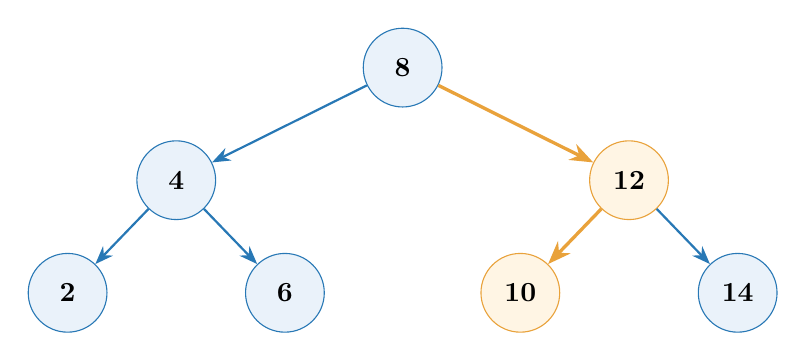
\begin{tikzpicture}[x=1.15cm,y=1.1cm,
v/.style={circle,draw=Blue,fill=PaleBlue,minimum size=10mm,font=\bfseries},
edge/.style={-{Stealth},thick,draw=Blue}]
\node[v] (a) at (0,0) {8};
\node[v] (b) at (-2.5,-1.3) {4};
\node[v,draw=Amber,fill=PaleAmber] (c) at (2.5,-1.3) {12};
\node[v] (d) at (-3.7,-2.6) {2};
\node[v] (e) at (-1.3,-2.6) {6};
\node[v,draw=Amber,fill=PaleAmber] (f) at (1.3,-2.6) {10};
\node[v] (g) at (3.7,-2.6) {14};
\draw[edge] (a)--(b); \draw[edge,draw=Amber,very thick] (a)--(c);
\draw[edge] (b)--(d); \draw[edge] (b)--(e);
\draw[edge,draw=Amber,very thick] (c)--(f); \draw[edge] (c)--(g);
\end{tikzpicture}

{\small 图2：二叉搜索树示例；琥珀色边表示查找10的路径。}
\end{center}

\subsection{一次成功查找：目标键10}
目标键记为$q$，当前节点的键记为$k$。比较$q$与$k$后，整个不可能包含目标的子树可以被排除。

\par\noindent\begin{tabularx}{\textwidth}{C{1cm}C{1.5cm}Y Y}
\toprule
步数 & 当前键 & 比较与行动 & 为什么可以排除另一侧\\
\midrule
1 & 8 & $10>8$，走右子树 & 左子树所有键均小于8\\
2 & 12 & $10<12$，走左子树 & 右子树所有键均大于12\\
3 & 10 & $10=10$，找到并停止 & 返回保存该键的节点\\
\bottomrule
\end{tabularx}\par

\subsection{一次失败查找：目标键11}
访问序列为8$\to$12$\to$10。到10时，$11>10$，还应去右孩子，但右孩子不存在，于是返回“未找到”。\textbf{到达叶节点不一定成功，必须检查键是否相等。}

\begin{questionbox}[思考题2]
若把键9放在节点4的右孩子位置，只检查“$9>4$”是否足够？
\end{questionbox}

\clearpage
\subsection{从查找路径到可执行循环}
以下代码只负责查找。假设每个节点对象已有\texttt{key}、\texttt{left}、\texttt{right}三个属性，空孩子为\texttt{None}；它不是配套决策树类的方法。
\begin{Verbatim}[frame=single,framesep=2mm,fontsize=\small,baselinestretch=1]
def search(root, target):
    node = root
    while node is not None:
        if target == node.key:
            return node
        if target < node.key:
            node = node.left
        else:
            node = node.right
    return None
\end{Verbatim}
\texttt{root}是树的入口，\texttt{target}是要找的键，\texttt{node}记录当前访问位置。\texttt{return}立即结束查找；\texttt{node = node.left}只移动当前引用，不删除右子树，也不修改原树。

\begin{proofbox}[为什么不会漏掉已存在的键]
每次进入循环时，若目标在树中，它一定在当前节点或当前子树里。若目标小于当前键，右子树的所有键都更大，可以整体排除；反之亦然。因此每次移动后，目标若存在，仍在保留下来的子树中。最终找到相等键，或者走到空位置证明不存在。
\end{proofbox}

\subsection{查找快不快，取决于树高}
设树中有$m$个节点，高度为$h$。每访问一个节点只做常数次比较，一条根到叶的路径最多访问$h+1$个节点。用$O(\cdot)$表示忽略常数后的增长量级：
\begin{equation}
T_{\mathrm{search}}=O(h+1).
\end{equation}
若树保持平衡，高度随节点数按对数增长；若把递增的键依次插入普通二叉搜索树，又不做平衡调整，树可能退化为链：
\begin{equation}
\text{平衡时： }h=O(\log m),\quad T_{\mathrm{search}}=O(\log m);
\qquad
\text{链状时： }h=m-1,\quad T_{\mathrm{search}}=O(m).
\end{equation}
\begin{center}
\begin{tikzpicture}[v/.style={draw=Blue,fill=PaleBlue,minimum size=8mm},arr/.style={-{Stealth},draw=Blue,thick}]
\node[v] (a) at (0,0) {1};
\node[v] (b) at (2,0) {2};
\node[v] (c) at (4,0) {3};
\node[v] (d) at (6,0) {4};
\draw[arr] (a)--node[above,font=\small]{右孩子}(b);
\draw[arr] (b)--node[above,font=\small]{右孩子}(c);
\draw[arr] (c)--node[above,font=\small]{右孩子}(d);
\end{tikzpicture}

{\small 图3：横向绘制的退化链，画法不改变父子关系。}
\end{center}
\begin{pitfallbox}
二叉搜索树的查找时间取决于树高；只有在树保持平衡时，才能保证对数级的查找时间。
\end{pitfallbox}

\clearpage
\section{决策树：把分支规则用于分类}
\subsection{从“找一个已有键”换成“判断一个新样本”}
西瓜分类的输入是一只瓜的属性，输出是类别。我们不要求新瓜与训练记录中的某只瓜完全相同，也不是用西瓜编号找到一个已有标签。需要的是一套能够应用到新属性组合上的判断规则。

\begin{center}
\begin{tikzpicture}[b/.style={draw=Blue,fill=PaleBlue,rounded corners,minimum width=3.7cm,minimum height=1cm,align=center},
a/.style={-{Stealth},thick,draw=Blue}]
\node[b] (x) at (0,0) {输入属性\\色泽、根蒂、纹理等};
\node[b] (t) at (5,0) {逐节点回答问题\\例如：纹理是什么？};
\node[b,draw=Cyan,fill=PaleCyan] (y) at (10,0) {到达叶节点\\输出好瓜或坏瓜};
\draw[a] (x)--(t); \draw[a] (t)--(y);
\end{tikzpicture}

{\small 图4：分类推理只读取属性；真实类别在预测完成后才用于核对。}
\end{center}

\par\noindent\begin{tabularx}{\textwidth}{L{2.6cm}Y Y}
\toprule
比较项 & 二叉搜索树 & 分类决策树\\
\midrule
要解决的问题 & 某个键是否已存在，在哪里 & 新样本应属于哪个类别\\
内部节点保存 & 可比较的键 & 一个属性测试或划分条件\\
分支由什么决定 & 目标键与当前键的大小 & 样本在测试属性上的取值\\
成功／停止位置 & 键相等；或走到空位置 & 到达叶节点；或使用默认回退\\
结构的来源 & 数据结构的构造与维护 & 从训练样本和标签中学习\\
是否必须二叉 & 是 & 不一定；可二叉，也可多叉\\
\bottomrule
\end{tabularx}\par

\subsection{训练与推理是两个不同阶段}
\term{训练}看到属性和标签，要决定“在哪个节点问哪个问题、何时停止、叶节点输出什么”。\term{推理}使用固定树，只看到待预测样本的属性，按现有分支走到答案；它不在每一步重新计算信息增益。

\begin{keybox}
本课使用\textbf{离散属性多叉决策树}：纹理有清晰、稍糊、模糊三种取值，就可以产生三个分支。二叉树是理解树结构的入口，不是对决策树分支数的限制。
\end{keybox}

\clearpage
\subsection{一棵可以执行的西瓜决策树}
图5由西瓜数据集的17条记录训练得到。浅蓝节点表示属性测试，浅青节点表示输出类别；边上的文字是属性取值。琥珀色边标出原编号15的推理路径。

\begin{center}
\begin{tikzpicture}[x=1.05cm,y=1.05cm,
test/.style={draw=Blue,fill=PaleBlue,rounded corners=.7mm,minimum width=1.35cm,minimum height=8mm,font=\small\bfseries},
leaf/.style={draw=Cyan,fill=PaleCyan,rounded corners=3mm,minimum width=1.3cm,minimum height=8mm,font=\small},
arr/.style={-{Stealth[length=2mm]},draw=Blue,thick},
path/.style={arr,draw=Amber,very thick},
lab/.style={font=\small,fill=white,inner sep=1pt}]
\node[test] (r) at (0,0) {纹理};
\node[test] (a) at (-3,-1.7) {根蒂};
\node[test] (b) at (2,-1.7) {触感};
\node[leaf] (c) at (5.3,-1.7) {坏瓜0};
\node[leaf] (d) at (-5.3,-3.5) {坏瓜0};
\node[leaf] (e) at (-3.3,-3.5) {好瓜1};
\node[test] (f) at (-1,-3.5) {色泽};
\node[leaf] (g) at (2,-3.5) {坏瓜0};
\node[leaf] (h) at (4.3,-3.5) {好瓜1};
\node[leaf] (i) at (-3.4,-5.3) {好瓜1};
\node[test] (j) at (-1,-5.3) {触感};
\node[leaf] (k) at (-2.6,-7.1) {好瓜1};
\node[leaf] (l) at (.6,-7.1) {坏瓜0};
\draw[path] (r)--node[lab,above left]{清晰}(a);
\draw[arr] (r)--node[lab,above right]{稍糊}(b);
\draw[arr] (r)--node[lab,above,sloped]{模糊}(c);
\draw[arr] (a)--node[lab,above left]{硬挺}(d);
\draw[arr] (a)--node[lab,right]{蜷缩}(e);
\draw[path] (a)--node[lab,above right]{稍蜷}(f);
\draw[arr] (b)--node[lab,left]{硬滑}(g);
\draw[arr] (b)--node[lab,above right]{软粘}(h);
\draw[arr] (f)--node[lab,above left]{青绿}(i);
\draw[path] (f)--node[lab,right]{乌黑}(j);
\draw[arr] (j)--node[lab,above left]{硬滑}(k);
\draw[path] (j)--node[lab,above right]{软粘}(l);
\node[align=left,font=\small,color=Muted] at (3.3,-5.8) {浅蓝矩形：读取一个属性\\浅青圆角：输出类别\\琥珀色线：本次访问路径};
\end{tikzpicture}

{\small 图5：西瓜分类决策树；划分准则与并列处理见第\ref{sec:feature-selection}节。}
\end{center}
\begin{questionbox}[思考题3]
原编号9的瓜，纹理为稍糊、触感为硬滑。需要读取色泽吗？
\end{questionbox}

\clearpage
\subsection{一次完整推理：先遮住标签，再走路径}
从表4.1取原编号15，只向预测函数提供六个属性：
\begin{equation}
\mathbf x=(\text{乌黑},\text{稍蜷},\text{浊响},\text{清晰},\text{稍凹},\text{软粘})^\top.
\end{equation}
这里$\mathbf x$是六维属性向量；$\top$表示转置，写成列向量便于统一数学记号。代码里仍用长度为6的列表表示一个样本，列编号从0开始。

\par\noindent\begin{tabularx}{\textwidth}{C{.9cm}L{2cm}L{2.8cm}Y}
\toprule
步骤 & 当前节点 & 读取的属性 & 进入的节点与输出\\
\midrule
1 & 纹理（列3） & \texttt{x[3]}为清晰 & 进入根蒂节点\\
2 & 根蒂（列1） & \texttt{x[1]}为稍蜷 & 进入色泽节点\\
3 & 色泽（列0） & \texttt{x[0]}为乌黑 & 进入触感节点\\
4 & 触感（列5） & \texttt{x[5]}为软粘 & 到坏瓜叶节点；输出0\\
\bottomrule
\end{tabularx}\par
\begin{keybox}
预测类别记为$\hat y$，帽号表示模型预测。该样本得到$\hat y=0$，与真实标签$y=0$相同。这里使用训练记录演示路径，属于训练集回代。
\end{keybox}

\subsection{未出现过的属性值怎样处理}
每个节点除属性列和分支字典外，还保存该节点训练样本中的\term{多数类}。预测时若找不到对应分支，本实验返回\textbf{当前节点}的多数类。

例如，沿“清晰$\to$稍蜷”到达色泽节点后，若新瓜色泽为该节点没见过的“浅白”，该节点的训练样本为原编号6、8、15，标签为1、1、0，因此回退输出1。回退不等于宣称该新瓜一定是好瓜；它只是数据不足时的默认决策。

\begin{pitfallbox}
当前节点的多数类可能与根节点不同。本例根节点8个好瓜、9个坏瓜，多数类为0；刚才色泽节点的多数类却为1。不能把所有未知分支都统一送回根节点的多数类。
\end{pitfallbox}
一次预测只访问从根出发的一条路径，访问长度决定推理的工作量。

\clearpage
\section{训练数据：把一筐瓜写成表}
\subsection{完整西瓜数据集2.0}
表1取自《机器学习》第4章表4.1，17条记录和6个离散属性全部保留；只把“是／否”编码为1／0。编号用于追溯教材，不参加划分。
\begin{center}
{\small
\begin{tabular}{cccccccc}
\toprule
原编号 & 色泽 & 根蒂 & 敲声 & 纹理 & 脐部 & 触感 & 好瓜\\
\midrule
1 & 青绿 & 蜷缩 & 浊响 & 清晰 & 凹陷 & 硬滑 & 1\\
2 & 乌黑 & 蜷缩 & 沉闷 & 清晰 & 凹陷 & 硬滑 & 1\\
3 & 乌黑 & 蜷缩 & 浊响 & 清晰 & 凹陷 & 硬滑 & 1\\
4 & 青绿 & 蜷缩 & 沉闷 & 清晰 & 凹陷 & 硬滑 & 1\\
5 & 浅白 & 蜷缩 & 浊响 & 清晰 & 凹陷 & 硬滑 & 1\\
6 & 青绿 & 稍蜷 & 浊响 & 清晰 & 稍凹 & 软粘 & 1\\
7 & 乌黑 & 稍蜷 & 浊响 & 稍糊 & 稍凹 & 软粘 & 1\\
8 & 乌黑 & 稍蜷 & 浊响 & 清晰 & 稍凹 & 硬滑 & 1\\
9 & 乌黑 & 稍蜷 & 沉闷 & 稍糊 & 稍凹 & 硬滑 & 0\\
10 & 青绿 & 硬挺 & 清脆 & 清晰 & 平坦 & 软粘 & 0\\
11 & 浅白 & 硬挺 & 清脆 & 模糊 & 平坦 & 硬滑 & 0\\
12 & 浅白 & 蜷缩 & 浊响 & 模糊 & 平坦 & 软粘 & 0\\
13 & 青绿 & 稍蜷 & 浊响 & 稍糊 & 凹陷 & 硬滑 & 0\\
14 & 浅白 & 稍蜷 & 沉闷 & 稍糊 & 凹陷 & 硬滑 & 0\\
15 & 乌黑 & 稍蜷 & 浊响 & 清晰 & 稍凹 & 软粘 & 0\\
16 & 浅白 & 蜷缩 & 浊响 & 模糊 & 平坦 & 硬滑 & 0\\
17 & 青绿 & 蜷缩 & 沉闷 & 稍糊 & 稍凹 & 硬滑 & 0\\
\bottomrule
\end{tabular}}

{\small 表1：原编号1--8是好瓜，9--17是坏瓜；代码保留上述行序。}
\end{center}

\subsection{样本、列和标签的记号}
训练集记为$D$，第$n$个样本为$\mathbf x^{(n)}$，标签为$y^{(n)}\in\{0,1\}$。括号上标$(n)$仅表示当前样本编号，不是幂；$x_j^{(n)}$表示其第$j$个属性。本讲义的属性列与Python一致，从0到5编号。

特征表$\mathbf X$按样本行排列，形状为$N\times d$；这里$N=17,d=6$。代码中用二维列表保存$\mathbf X$，每项是表示离散属性值的字符串。标签向量$\mathbf y$长度为17。当前数学样本编号从1起，Python行索引从0起；抽取子集后，子集当前行号与教材原编号要分开保存。

下文$D$也表示正在处理的节点样本子集，其大小随递归改变。

\clearpage
\section{信息熵：衡量节点还剩多少不确定性}
\subsection{先有类别比例，再有熵}
若一个节点里的瓜全是好瓜，已经不需要再问；若好坏各半，单凭这个节点还难以判断。先用当前节点内的经验比例表示类别分布。记$p_k$为类别$k$所占比例，$k=0,1$；$|D|$表示样本数，$\#\{\cdot\}$表示满足条件的计数：
\begin{equation}
p_k=\frac{\#\{n:y^{(n)}=k,\ \mathbf x^{(n)}\text{属于当前节点}\}}{|D|},
\qquad p_0+p_1=1.
\end{equation}
类别概率为$p$的结果，用$-\log_2p$表示它出现时的信息量：越罕见，信息量越大。$\log_2$是以2为底的对数，单位为比特（bit）。按结果出现的概率求平均，就得到\term{信息熵}：
\begin{equation}
\operatorname{Ent}(D)=\sum_{k=0}^{1}p_k(-\log_2p_k)
=-\sum_{k=0}^{1}p_k\log_2p_k.
\end{equation}
$\operatorname{Ent}$是把标签分布映射为非负数的函数；$\sum$表示对两个类别的项求和。约定$0\log_2 0=0$，程序中跳过概率为0的项，不计算\texttt{log2(0)}。

\subsection{三组能手算的标签}
\par\noindent\begin{tabularx}{\textwidth}{L{3.1cm}L{3.2cm}Y}
\toprule
标签 & 类别比例 & 熵与解释\\
\midrule
$[1,1,1,1]$ & $p_1=1,\ p_0=0$ & 熵为0，纯节点\\
$[0,0,1,1]$ & $p_1=p_0=1/2$ & 熵为1，二分类最不确定\\
$[0,0,0,1]$ & $p_1=1/4,\ p_0=3/4$ & 熵约0.811278，比均分更纯\\
\bottomrule
\end{tabularx}\par
对西瓜数据集中的17条训练记录：
\begin{equation}
\operatorname{Ent}(D)
=-\frac8{17}\log_2\frac8{17}-\frac9{17}\log_2\frac9{17}
\approx0.997502546.
\end{equation}
\begin{keybox}
二分类熵介于0与1之间，越小越纯。熵不是“好瓜概率”：全是坏瓜与全是好瓜的熵都为0，但输出类别不同。因此节点还需另存类别信息。
\end{keybox}
\begin{questionbox}[思考题4]
把$[0,0,1,1]$的最后一个1改成0，熵变大还是变小？
\end{questionbox}

\clearpage
\section{信息增益：选哪个问题最有帮助}
\subsection{从分支概率推出加权平均}
选属性列$j$提问时，令$V_j$表示该属性在当前节点实际出现的不同取值集合；例如纹理的集合为$\{\text{清晰},\text{稍糊},\text{模糊}\}$。令$D_{j=v}$表示属性$j$取值为$v$的样本子集。

从当前节点均匀抽一条记录，它落入分支$v$的比例为$|D_{j=v}|/|D|$。已知分支后的剩余不确定性为$\operatorname{Ent}(D_{j=v})$，因此提问后的平均不确定性是
\begin{equation}
H_{\mathrm{after}}(D,j)
=\sum_{v\in V_j}\frac{|D_{j=v}|}{|D|}\operatorname{Ent}(D_{j=v}).
\end{equation}
这里$H_{\mathrm{after}}$是当前属性划分后的加权熵，输入是当前节点与属性列，输出仍以bit为单位。各分支权重之和为1。\term{信息增益}就是划分前后不确定性的减少：
\begin{equation}
\operatorname{Gain}(D,j)
=\operatorname{Ent}(D)-H_{\mathrm{after}}(D,j)
=\operatorname{Ent}(D)
-\sum_{v\in V_j}\frac{|D_{j=v}|}{|D|}\operatorname{Ent}(D_{j=v}).
\end{equation}

\begin{proofbox}[为什么不能把几个分支直接平均]
设一个分支只有1条样本，另一个有16条；它们分别影响原节点的$1/17$与$16/17$。直接取两个熵的算术平均，会把那个只有1条样本的分支放大到一半权重。按样本数加权，才对应“随机抽取一个当前样本，问完问题后平均还剩多少不确定性”。
\end{proofbox}

\subsection{把数学目标变成一次属性搜索}\label{sec:feature-selection}
令$A$为当前路径还没有使用的候选属性列集合，$j^*$表示选择结果；$\arg\max$返回使增益最大的\textbf{属性编号}，不是增益值：
\begin{equation}
j^*=\operatorname*{arg\,max}_{j\in A,\ |V_j|>1}\operatorname{Gain}(D,j).
\end{equation}
只考虑能形成至少两个非空分支的属性；增益并列时按候选列表顺序选先遇到者。程序将相差不超过$10^{-12}$视作并列，减轻浮点计算差异。

这一步是\term{贪心选择}：只优化当前节点的一步划分，不保证整棵树最浅或测试误差最小。以信息增益选择属性的经典方法称为ID3（Iterative Dichotomiser 3）；本实验实现其中的离散属性递归划分主线。

\begin{questionbox}[思考题5]
某个属性在当前节点全部相同，它的增益是多少？
\end{questionbox}

\clearpage
\subsection{根节点手算：纹理的三条分支}
回到完整的17条记录。先按纹理分组，再分别计数和计算熵。表中编号均为教材原编号。
\par\noindent\begin{tabularx}{\textwidth}{L{1.15cm}Y C{.9cm}C{.9cm}C{1.25cm}L{2.2cm}}
\toprule
纹理 & 原编号 & 好瓜 & 坏瓜 & 权重 & 子节点熵\\
\midrule
清晰 & 1、2、3、4、5、6、8、10、15 & 7 & 2 & $9/17$ & 0.764204507\\
稍糊 & 7、9、13、14、17 & 1 & 4 & $5/17$ & 0.721928095\\
模糊 & 11、12、16 & 0 & 3 & $3/17$ & 0\\
\bottomrule
\end{tabularx}\par
以清晰分支为例，将7个好瓜、2个坏瓜代入：
\begin{equation}
\operatorname{Ent}(D_{3=\text{清晰}})
=-\frac79\log_2\frac79-\frac29\log_2\frac29
\approx0.764204507.
\end{equation}
其余两支分别得到$-\frac15\log_2\frac15-\frac45\log_2\frac45\approx0.721928095$和0。用分支样本比例加权：
\begin{equation}
\begin{aligned}
H_{\mathrm{after}}(D,3)
&\approx\frac9{17}\times0.764204507
+\frac5{17}\times0.721928095+\frac3{17}\times0\\
&\approx0.616910649,\\
\operatorname{Gain}(D,3)
&\approx0.997502546-0.616910649
=0.380591897.
\end{aligned}
\end{equation}
这里3是纹理的Python列编号。对六个属性做同样的计算：
\begin{center}
\begin{tabular}{lrrrrrr}
\toprule
属性 & 色泽 & 根蒂 & 敲声 & 纹理 & 脐部 & 触感\\
\midrule
原始计数计算值 & .108125 & .142675 & .140781 & \textbf{.380592} & .289159 & .006046\\
教材列示近似值 & .109 & .143 & .141 & \textbf{.381} & .289 & .006\\
\bottomrule
\end{tabular}
\end{center}
\begin{keybox}
六个属性中，纹理的信息增益最大，因此选择纹理作为根节点的划分属性。
\end{keybox}
\noindent{\small\textbf{数值说明：}用原始计数计算，色泽增益约为0.108125；若先将各熵保留三位小数，再计算并舍入，可得教材列示的0.109。程序按原始计数计算。\par}

\clearpage
\subsection{再走一层：必须在子集内重新计算}
根节点选纹理后，“模糊”分支全是坏瓜，立即成为叶节点；“清晰”分支还有9条记录，包含7个好瓜和2个坏瓜，仍需划分。记这个子集为$D_{\mathrm{clear}}$，可用属性不再包含纹理。

若按根蒂分组，会得到：
\par\noindent\begin{tabularx}{\textwidth}{L{1.5cm}Y L{2.6cm}L{2.5cm}}
\toprule
根蒂 & 原编号 & 标签计数 & 子节点熵\\
\midrule
蜷缩 & 1、2、3、4、5 & 好5、坏0 & 0\\
稍蜷 & 6、8、15 & 好2、坏1 & 0.918295834\\
硬挺 & 10 & 好0、坏1 & 0\\
\bottomrule
\end{tabularx}\par
因此，根蒂在当前子集中的增益为
\begin{equation}
\begin{aligned}
\operatorname{Gain}(D_{\mathrm{clear}},1)
&\approx0.764204507
-\left(\frac59\times0+\frac39\times0.918295834+\frac19\times0\right)\\
&\approx0.458105895.
\end{aligned}
\end{equation}
注意这里权重的分母为\textbf{9}，不是根节点的17。重新计算剩余属性得到：
\begin{center}
\begin{tabular}{lrrrrr}
\toprule
属性 & 色泽 & 根蒂 & 敲声 & 脐部 & 触感\\
\midrule
当前增益 & .043068 & \textbf{.458106} & .330856 & \textbf{.458106} & \textbf{.458106}\\
\bottomrule
\end{tabular}
\end{center}
根蒂、脐部和触感的增益并列，按候选列顺序选择根蒂。选择其他并列最优属性时，可能得到不同的树形。

\subsection{后续节点的划分}
沿“清晰$\to$稍蜷”剩下原编号6、8、15，标签为1、1、0，熵约0.918296。此时色泽与触感的增益都约为0.251629，优先选色泽；乌黑分支剩下8、15，最后由触感区分为好瓜与坏瓜。这样就得到图5中原编号15走过的那条路径。

\begin{questionbox}[思考题6]
能否先在完整数据上把六个属性排好序，然后每一层照这个顺序提问？
\end{questionbox}

\clearpage
\section{从公式到算法：递归训练与循环预测}
\subsection{叶节点为什么使用多数类}
某个节点无法继续细分时，必须用一个类别代表其中全部记录。设候选输出为$c\in\{0,1\}$；$\mathbf1[\cdot]$是指示函数，条件成立取1，否则取0。当前节点的错误数为
\begin{equation}
E_D(c)=\sum_{\mathbf x^{(n)}\in D}\mathbf1[y^{(n)}\ne c]
=|D|-\#\{n:y^{(n)}=c,\ \mathbf x^{(n)}\in D\}.
\end{equation}
因此，使错误数最小就等价于使正确类的计数最大：
\begin{equation}
c^*=\operatorname*{arg\,min}_{c\in\{0,1\}}E_D(c)
=\operatorname*{arg\,max}_{c\in\{0,1\}}\#\{n:y^{(n)}=c,\ \mathbf x^{(n)}\in D\}.
\end{equation}
$\arg\min$表示取到最小值的类别；这就是多数类规则的来由。这里默认两种误判代价相同；平票时本实验固定选0，便于复现。

\subsection{训练：把同一个任务交给更小的子集}
\begin{enumerate}
\item 创建默认叶节点，记录当前多数类。
\item 若标签已经全相同，直接返回；若候选属性为空，也直接返回。
\item 在当前子集上搜索有至少两种取值的候选属性，选信息增益最大的一个。若没有可划分属性，返回默认叶节点。
\item 把该属性记录为当前节点的问题。对实际出现的每个取值，取出对应特征行与标签。
\item 用新的候选属性列表递归建子树：只去掉已经使用的属性编号，保留特征矩阵所有列；把返回的子树挂到该取值的分支下。
\end{enumerate}
递归是在更小子集上调用同一个建树方法。每条路径至多使用6个离散属性，因此会结束；纯节点和无法细分的节点还会提前结束。

\begin{pitfallbox}
不要额外加入“增益为0就立即停止”的规则。人工构造的两位异或数据$(0,0)\mapsto0$、$(0,1)\mapsto1$、$(1,0)\mapsto1$、$(1,1)\mapsto0$，两个属性在根处的增益都为0，但先划分一个，再划分另一个就能分开全部类别。
\end{pitfallbox}
\begin{notebox}
本实现只为当前节点实际出现的属性值创建分支，因此递归不接收空子集。预测时遇到未知属性值，按第4.5节的规则回退。这一约定用于默认分类，尚未处理训练数据中的缺失值。
\end{notebox}

\clearpage
\subsection{与Python类骨架逐一对照}
\par\noindent\begin{tabularx}{\textwidth}{L{4.3cm}Y L{2cm}}
\toprule
方法 & 职责 & 手敲顺序\\
\midrule
\texttt{\_\_init\_\_} & 初始化根节点，暂不训练 & 已提供\\
\texttt{\_entropy(y)} & 计数、求比例、累加负对数项 & T1\\
\texttt{\_majority\_label(y)} & 返回多数类，平票选0 & T2\\
\texttt{\_information\_gain} & 分组并计算加权熵减少量 & T3\\
\texttt{\_best\_feature} & 比较当前可用属性的增益 & T4\\
\texttt{\_build\_tree} & 判断终止条件，递归创建子树 & T5\\
\texttt{fit(X, y)} & 保存训练得到的根节点 & 已提供\\
\texttt{\_predict\_one(x)} & 对一个样本沿分支走到输出 & T6\\
\texttt{predict(X)} & 按输入行序重复单样本预测 & T7\\
\bottomrule
\end{tabularx}\par

\subsection{单样本预测的实现}
在T6的\texttt{\_predict\_one}中，将图5的预测路径写成循环：
\begin{enumerate}
\item 令当前节点为\texttt{self.root}。
\item 若当前节点为叶节点，返回其\texttt{label}。
\item 读取当前节点保存的属性列编号，再取出样本\texttt{x}在该列的值。
\item 若该值对应的分支不存在，返回当前节点的\texttt{label}；否则进入对应子节点，继续循环。
\end{enumerate}
输入\texttt{x}是一个样本的完整特征列表，输出是0或1。调用前必须完成训练；内部节点保存原始属性列编号，叶节点的\texttt{feature}为\texttt{None}。完成T6后，再在T7中按输入行序重复调用单样本预测。

\begin{questionbox}[思考题7]
这一循环与二叉搜索树的查找循环有什么共同点、什么不同点？
\end{questionbox}
\textbf{易错提醒：}列0是合法属性，必须判断\texttt{feature is None}。训练时保留$\mathbf X$的列，避免原始列编号错位。

\clearpage
\section{评估与局限：长出一棵树还不够}
\subsection{回代正确，不等于新样本正确}
图5可以将当前17条训练记录全部分对。用训练时见过的记录再次预测，称为训练集回代；这个结果可用于检查实现，但不能说明模型对未见样本的预测表现。

\par\noindent\begin{tabularx}{\textwidth}{L{2.4cm}Y Y}
\toprule
数据部分 & 允许的用途 & 不应承担的用途\\
\midrule
训练集 & 学习属性划分、分支与叶类别 & 不能用回代成绩替代独立评价\\
验证集 & 选择最大深度或剪枝等方案 & 不能把方案选择后的分数当最终证据\\
测试集 & 方案锁定后评价新样本表现 & 不能反复用于选属性、调参或删难例\\
\bottomrule
\end{tabularx}\par
本课主线只实现离散树且不剪枝；剪枝是删除收益不足的分支来控制复杂度。将来比较剪枝方案时，应预先留出验证集，不用测试集挑出“最好看”的树。

\subsection{准确率与误判代价}
对独立评价集$D_{\mathrm{eval}}$，样本数为$N_{\mathrm{eval}}$，预测类别为$\hat y^{(n)}$。准确率对所有样本的预测是否正确求平均：
\begin{equation}
\operatorname{Accuracy}
=\frac1{N_{\mathrm{eval}}}\sum_{n=1}^{N_{\mathrm{eval}}}
\mathbf1[\hat y^{(n)}=y^{(n)}].
\end{equation}
帽号仍表示预测，$\mathbf1$仍是指示函数。若卖瓜时“坏瓜判为好瓜”的代价更高，应分别统计两类误判，不能只看一个准确率。多数类叶节点的规则也隐含了等代价假设。

\subsection{需要记住的局限}
\begin{itemize}
\item 信息增益偏好取值多的属性。若把唯一编号作为属性，每个分支只有一条记录，熵会变为0，却只记住了训练样本。
\item 小样本稍有变化，最大增益属性和树结构就可能改变；并列最优时树也不唯一。
\item 很深的树容易拟合训练噪声。不断减少训练熵不保证减少测试错误。
\item 本实现只处理离散属性。连续特征需要搜索阈值；不能把每个不同小数直接当成一个分支来替代阈值学习。
\end{itemize}

\clearpage
\section{练习与参考解答}
\subsection{自测题}
\begin{enumerate}
\item 一棵树每个节点有至多两个孩子，就一定是二叉搜索树吗？请给理由。
\item 预测一条新样本时，程序需要访问整棵决策树吗？需要读取训练集或真实标签吗？
\item 分支大小不同，为什么信息增益公式不能直接平均子节点熵？
\item 某个叶节点的训练标签为$[1,1,0]$，按多数类规则输出什么？此时会错分几条训练记录？
\end{enumerate}

\subsection{课后练习：从手算到程序}
\begin{enumerate}
\item 在图2中分别查找6和5，写出访问序列与停止原因。若树有7个节点，它是否一定只比较3次？
\item 教学标签集合为$[0,0,0,1]$。求信息熵；再按某属性划成$[0,0]$与$[0,1]$，求加权子熵和信息增益。
\item 不看答案，用表1复核纹理的三组计数及信息增益；指出哪条分支立即成为叶节点。
\item 一条样本的纹理为清晰、根蒂为稍蜷、色泽为乌黑，触感为未见过的“粗糙”。沿图5写出预测路径，并根据到达节点的训练记录判断输出类别。
\item 完成配套脚本T1--T3，运行脚本并对照手算结果；说明\texttt{count/len(y)}、\texttt{log2}、分支权重各对应哪个数学量。再继续完成T4--T7。
\end{enumerate}
\begin{notebox}[调试建议]
可在信息增益分组处和递归入口设置断点，检查当前标签、样本数和候选列。每完成一个方法，先用小样例确认输出，再运行完整数据。
\end{notebox}

\clearpage
\subsection{课后练习参考解答}
\begin{examplebox}[练习1：查找6和5]
查找6：8$\to$4$\to$6，在键相等时成功。查找5：8$\to$4$\to$6，随后应去6的左孩子，该位置为空，所以失败。7个节点也可能组成高度6的链，最坏需访问7个节点；不能只凭节点数断言树保持平衡。
\end{examplebox}

\begin{examplebox}[练习2：加权减少量]
原标签比例为$3/4$和$1/4$，因此
\begin{equation}
\operatorname{Ent}(D)
=-\frac34\log_2\frac34-\frac14\log_2\frac14
\approx0.811278124.
\end{equation}
两个子集各有2条样本，熵分别为0和1，所以
\begin{equation}
H_{\mathrm{after}}=\frac24\times0+\frac24\times1=0.5,\qquad
\operatorname{Gain}\approx0.811278124-0.5=0.311278124.
\end{equation}
这里只有在两个子集大小相同时，加权平均恰好等于算术平均。
\end{examplebox}

\begin{examplebox}[练习3与4：回到真实数据]
纹理清晰分支为好7坏2，稍糊为好1坏4，模糊为好0坏3。三条分支的样本数分别为9、5、3，根处增益约0.380591897，模糊分支直接成为坏瓜叶节点。

练习4的路径为“纹理=清晰$\to$根蒂=稍蜷$\to$色泽=乌黑”，到达触感节点。该节点对应原编号8、15，标签分别为1、0；“粗糙”没有对应分支，两类平票时按约定输出0。这里使用触感节点的计数，而不是其父节点的多数类1。
\end{examplebox}

\begin{keybox}[练习5：公式与语句的映射]
\texttt{count/len(y)}得到$p_k$；\texttt{-p * log2(p)}是单类对熵的贡献；\texttt{len(child\_y)/len(y)}是当前分支权重。信息增益用父熵减去加权子熵。\texttt{y}必须始终是当前节点的标签，不能在递归中错用全体17条标签。
\end{keybox}

\clearpage
\clearpage
\subsection{思考题与自测题参考解答}
\textbf{思考题}
\begin{enumerate}
\item 6个节点、5条边、3个叶节点；不会，因为B仍有左孩子D。
\item 不够。9仍处在根8的左子树中，却大于8，违反了整棵子树的约束。
\item 不需要。按“纹理=稍糊”进入触感节点，再按“硬滑”到坏瓜叶节点。预测时只访问一条路径。
\item 变小，约为0.811278；某一类更占优势，剩余不确定性减少。
\item 0。唯一子集就是原集合，划分前后的熵相同，不能缩小问题。
\item 不能。各子集的类别比例、分支比例都变了，必须重新计算。原列顺序只用于并列时的确定性选择，不代替信息增益。
\item 都维护当前节点、依据规则移动并在适当位置停止。查找循环比较目标键与节点键；预测循环读取样本属性，根据分支字典移动，返回叶节点类别。
\end{enumerate}

\textbf{自测题}
\begin{enumerate}
\item 不一定。二叉搜索树还要求每个节点的左子树所有键都小于当前键，右子树所有键都大于当前键。
\item 只沿一条路径访问节点，直到输出类别；预测只需要已训练的树和新样本属性。
\item 每个分支对原节点的影响取决于它包含的样本比例，因此须用该比例加权。
\item 输出1，错分1条记录。在误判代价相同的前提下，多数类使当前节点的错误数最少。
\end{enumerate}

\clearpage
\section{符号索引与资料}
\subsection{数据与模型}
\par\noindent\begin{tabularx}{\textwidth}{L{3.2cm}Y L{2cm}}
\toprule
符号 & 含义 & 首次说明\\
\midrule
$q,k$ & 查找目标键、当前节点的键 & 3.2\\
$m,h$ & 搜索树节点数、高度；根深度为0 & 3.5\\
$\mathbf x,\mathbf x^{(n)}$ & 单个属性向量、第$n$个当前样本 & 4.4、5.2\\
$x_j^{(n)},y^{(n)},\hat y^{(n)}$ & 第$j$个属性、真实标签、预测标签 & 5.2、4.4\\
$\mathbf X,\mathbf y,N,d$ & 按行排列的特征、标签、样本数、属性数 & 5.2\\
$D,D_{j=v},V_j,A$ & 当前样本集、分支子集、取值集合、候选列 & 5.2、7.1--7.2\\
\bottomrule
\end{tabularx}\par
\subsection{函数、算子与经验比例}
\par\noindent\begin{tabularx}{\textwidth}{L{3.2cm}Y L{2cm}}
\toprule
符号 & 含义 & 首次说明\\
\midrule
$|D|,\#\{\cdot\}$ & 集合大小、满足条件的计数 & 6.1\\
$p_k$ & 当前节点内类别$k$的经验比例 & 6.1\\
$\log_2,\sum$ & 以2为底的对数、求和 & 6.1\\
$\operatorname{Ent},H_{\mathrm{after}}$ & 节点信息熵、划分后的加权熵 & 6.1、7.1\\
$\operatorname{Gain},j^*$ & 信息增益、选中的属性列 & 7.1--7.2\\
$\arg\max,\arg\min$ & 返回最大／最小函数值对应的参数 & 7.2、8.1\\
$\mathbf1[\cdot],E_D(c),c^*$ & 指示函数、错误数、所选叶类别 & 8.1\\
$\top,\hat{\phantom{y}},O(\cdot)$ & 转置、预测帽号、增长量级 & 4.4、3.5\\
$D_{\mathrm{eval}},N_{\mathrm{eval}}$ & 独立评价集及其样本数 & 9.2\\
\bottomrule
\end{tabularx}\par
\subsection{参考资料}
\begin{enumerate}
\item 周志华，《机器学习》，第4章：决策树。表4.1提供本讲义使用的西瓜数据；信息熵与信息增益用于选择划分属性。
\item 配套练习：\path{code/decision_tree.py}。
\item 语法复习：《Python语法带练》及\path{code/python_syntax/}中的分章脚本。
\end{enumerate}
\end{document}
